\documentclass[twoside]{book}

% Packages required by doxygen
\usepackage{fixltx2e}
\usepackage{calc}
\usepackage{doxygen}
\usepackage[export]{adjustbox} % also loads graphicx
\usepackage{graphicx}
\usepackage[utf8]{inputenc}
\usepackage{makeidx}
\usepackage{multicol}
\usepackage{multirow}
\PassOptionsToPackage{warn}{textcomp}
\usepackage{textcomp}
\usepackage[nointegrals]{wasysym}
\usepackage[table]{xcolor}

% Font selection
\usepackage[T1]{fontenc}
\usepackage[scaled=.90]{helvet}
\usepackage{courier}
\usepackage{amssymb}
\usepackage{sectsty}
\renewcommand{\familydefault}{\sfdefault}
\allsectionsfont{%
  \fontseries{bc}\selectfont%
  \color{darkgray}%
}
\renewcommand{\DoxyLabelFont}{%
  \fontseries{bc}\selectfont%
  \color{darkgray}%
}
\newcommand{\+}{\discretionary{\mbox{\scriptsize$\hookleftarrow$}}{}{}}

% Page & text layout
\usepackage{geometry}
\geometry{%
  a4paper,%
  top=2.5cm,%
  bottom=2.5cm,%
  left=2.5cm,%
  right=2.5cm%
}
\tolerance=750
\hfuzz=15pt
\hbadness=750
\setlength{\emergencystretch}{15pt}
\setlength{\parindent}{0cm}
\setlength{\parskip}{3ex plus 2ex minus 2ex}
\makeatletter
\renewcommand{\paragraph}{%
  \@startsection{paragraph}{4}{0ex}{-1.0ex}{1.0ex}{%
    \normalfont\normalsize\bfseries\SS@parafont%
  }%
}
\renewcommand{\subparagraph}{%
  \@startsection{subparagraph}{5}{0ex}{-1.0ex}{1.0ex}{%
    \normalfont\normalsize\bfseries\SS@subparafont%
  }%
}
\makeatother

% Headers & footers
\usepackage{fancyhdr}
\pagestyle{fancyplain}
\fancyhead[LE]{\fancyplain{}{\bfseries\thepage}}
\fancyhead[CE]{\fancyplain{}{}}
\fancyhead[RE]{\fancyplain{}{\bfseries\leftmark}}
\fancyhead[LO]{\fancyplain{}{\bfseries\rightmark}}
\fancyhead[CO]{\fancyplain{}{}}
\fancyhead[RO]{\fancyplain{}{\bfseries\thepage}}
\fancyfoot[LE]{\fancyplain{}{}}
\fancyfoot[CE]{\fancyplain{}{}}
\fancyfoot[RE]{\fancyplain{}{\bfseries\scriptsize Generated by Doxygen }}
\fancyfoot[LO]{\fancyplain{}{\bfseries\scriptsize Generated by Doxygen }}
\fancyfoot[CO]{\fancyplain{}{}}
\fancyfoot[RO]{\fancyplain{}{}}
\renewcommand{\footrulewidth}{0.4pt}
\renewcommand{\chaptermark}[1]{%
  \markboth{#1}{}%
}
\renewcommand{\sectionmark}[1]{%
  \markright{\thesection\ #1}%
}

% Indices & bibliography
\usepackage{natbib}
\usepackage[titles]{tocloft}
\setcounter{tocdepth}{3}
\setcounter{secnumdepth}{5}
\makeindex

% Hyperlinks (required, but should be loaded last)
\usepackage{ifpdf}
\ifpdf
  \usepackage[pdftex,pagebackref=true]{hyperref}
\else
  \usepackage[ps2pdf,pagebackref=true]{hyperref}
\fi
\hypersetup{%
  colorlinks=true,%
  linkcolor=blue,%
  citecolor=blue,%
  unicode%
}

% Custom commands
\newcommand{\clearemptydoublepage}{%
  \newpage{\pagestyle{empty}\cleardoublepage}%
}

\usepackage{caption}
\captionsetup{labelsep=space,justification=centering,font={bf},singlelinecheck=off,skip=4pt,position=top}

%===== C O N T E N T S =====

\begin{document}

% Titlepage & ToC
\hypersetup{pageanchor=false,
             bookmarksnumbered=true,
             pdfencoding=unicode
            }
\pagenumbering{roman}
\begin{titlepage}
\vspace*{7cm}
\begin{center}%
{\Large Duplicate File Remover }\\
\vspace*{1cm}
{\large Generated by Doxygen 1.8.11}\\
\end{center}
\end{titlepage}
\clearemptydoublepage
\tableofcontents
\clearemptydoublepage
\pagenumbering{arabic}
\hypersetup{pageanchor=true}

%--- Begin generated contents ---
\chapter{D\+U\+P\+L\+I\+C\+A\+TE F\+I\+LE R\+E\+M\+O\+V\+ER}
\label{index}\hypertarget{index}{}\href{https://github.com/vishal-wadhwa/Duplicate-File-Remover}{\tt Git\+Hub}

A command line utility that {\bfseries recursively} scans the set directory to find exact duplicate files inside all the sub-\/directories. The files so found can be listed in an output file. If required the duplicates can also be removed, thereby preserving a single unique file.

\href{https://asciinema.org/a/14}{\tt }

{\bfseries Features\+:}
\begin{DoxyEnumerate}
\item Recursive scan of the set directory.
\item Generate list of duplicate files.
\item Scan all files or filter based on file extension.
\end{DoxyEnumerate}

{\bfseries Future Plans\+:}
\begin{DoxyEnumerate}
\item Set a recursive scan depth for the set directory.
\item A way to exclude certain directories.
\item A way to include only some directories.
\item Robust error handling for synchronization issues.
\item Make the program interactive.
\end{DoxyEnumerate}

\begin{quote}
Caution\+: As of now, there is no way to select which of the duplicate files will be preserved. The selection happens on the order in which they are loaded into {\ttfamily std\+::map}. The first file is the one which is preserved. \end{quote}


\subsection*{\label{_dep}%
Dependencies\+:}


\begin{DoxyEnumerate}
\item For main program\+:

{\ttfamily sudo apt-\/get install libssl-\/dev libboost-\/filesystem-\/dev libboost-\/system-\/dev}
\item For tests, apart from the dependencies for main program\+:

{\ttfamily sudo apt-\/get install libcppunit-\/dev}
\end{DoxyEnumerate}

\subsection*{Downloading and Building}


\begin{DoxyEnumerate}
\item Clone the project\+:

{\ttfamily git clone \href{https://github.com/vishal-wadhwa/Duplicate-File-Remover.git}{\tt https\+://github.\+com/vishal-\/wadhwa/\+Duplicate-\/\+File-\/\+Remover.\+git}}
\item Change directory to src\+:

{\ttfamily cd Duplicate-\/\+File-\/\+Remover/src}
\item Build project using Make utility (assuming you\textquotesingle{}ve downloaded the \href{#dep}{\tt dependencies})\+:

{\ttfamily make main}
\item Run it (See \href{#use}{\tt Usage})\+:

{\ttfamily ./main ...}
\end{DoxyEnumerate}

\subsection*{Testing}


\begin{DoxyEnumerate}
\item From the root directory of the project go to tests directory\+:

{\ttfamily cd Duplicate-\/\+File-\/\+Remover/tests}
\item Build tests using Make utility (assuming you\textquotesingle{}ve downloaded the \href{#dep}{\tt dependencies})\+:

{\ttfamily make test}
\item Run them tests, bruh\+:

{\ttfamily ./test}
\end{DoxyEnumerate}

You should see {\itshape OK} if all the tests pass and then you can go on to using the program. ;)

\subsection*{\label{_use}%
Usage}


\begin{DoxyEnumerate}
\item Use {\ttfamily -\/d} switch to set the directory to be scanned.
\item Use {\ttfamily -\/e} switch to provide a list of extensions to filter the files scanned.
\item Use {\ttfamily -\/l} switch to generate an output(log) file. If this switch is not followed by a name/path, then a default file {\itshape dupl\+\_\+file.\+txt} is generated in the current directory.
\item Use {\ttfamily -\/r} switch to remove the duplicates and keep only one copy.
\item Use {\ttfamily -\/h} switch to display this help\+:
\end{DoxyEnumerate}


\begin{DoxyCode}
1 Usage: ./main -d [DIRECTORY]
2 or: ./main -d [DIRECTORY] -e [EXTENSIONS]...
3 or: ./main -d [DIRECTORY] -l [OUTFILE]
4 
5 Scan the provided directory and its sub-directories recursively and find duplicates.
6 
7 Not using either of -l or -r switch is pointless as no action is performed.
8 
9 -d switch is necessary to set the search directory.
10 
11 Other switches:
12     -d      provided argument is the directory to be scanned.
13     -e      following arguments treated as extensions.
14     -l      generate file list (default file: "dupl\_file.txt").
15     -h      prints this help.
16     -r      remove the duplicates so found.
\end{DoxyCode}
 \begin{quote}
Note\+: Use {\ttfamily sudo} if required. \end{quote}


\subsection*{Examples}


\begin{DoxyEnumerate}
\item {\ttfamily ./main -\/d ./ -\/l -\/r}
\item {\ttfamily ./main -\/e png jpg jpeg -\/d ./../ -\/l log.\+out}
\item {\ttfamily ./main -\/d ./ -\/r} 
\end{DoxyEnumerate}
\chapter{Class Index}
\section{Class List}
Here are the classes, structs, unions and interfaces with brief descriptions\+:\begin{DoxyCompactList}
\item\contentsline{section}{\hyperlink{structdfr_1_1file__data}{dfr\+::file\+\_\+data} }{\pageref{structdfr_1_1file__data}}{}
\item\contentsline{section}{\hyperlink{classdfr_1_1file__handler}{dfr\+::file\+\_\+handler} }{\pageref{classdfr_1_1file__handler}}{}
\item\contentsline{section}{\hyperlink{classdfr_1_1hash}{dfr\+::hash} }{\pageref{classdfr_1_1hash}}{}
\end{DoxyCompactList}

\chapter{File Index}
\section{File List}
Here is a list of all documented files with brief descriptions\+:\begin{DoxyCompactList}
\item\contentsline{section}{include/\hyperlink{file__handler_8h}{file\+\_\+handler.\+h} }{\pageref{file__handler_8h}}{}
\item\contentsline{section}{include/\hyperlink{file__hash_8h}{file\+\_\+hash.\+h} }{\pageref{file__hash_8h}}{}
\end{DoxyCompactList}

\chapter{Class Documentation}
\hypertarget{structdfr_1_1file__data}{}\section{dfr\+:\+:file\+\_\+data Struct Reference}
\label{structdfr_1_1file__data}\index{dfr\+::file\+\_\+data@{dfr\+::file\+\_\+data}}


{\ttfamily \#include $<$file\+\_\+handler.\+h$>$}

\subsection*{Public Member Functions}
\begin{DoxyCompactItemize}
\item 
\hyperlink{structdfr_1_1file__data_a7c0c7de83cd3104896d2e2b5a105bfab}{file\+\_\+data} (const std\+::string \&name, const uintmax\+\_\+t \&\hyperlink{structdfr_1_1file__data_a4fbf33ba9872a4fc575ef911e5a8f80c}{size}, const std\+::string \&\hyperlink{structdfr_1_1file__data_a49e1a762af0cfc8dd25669a1c17340da}{path})
\begin{DoxyCompactList}\small\item\em size of the file. \end{DoxyCompactList}\end{DoxyCompactItemize}
\subsection*{Public Attributes}
\begin{DoxyCompactItemize}
\item 
std\+::string {\bfseries name}\hypertarget{structdfr_1_1file__data_a9dd5c141e4c286b7443a1c08e656999f}{}\label{structdfr_1_1file__data_a9dd5c141e4c286b7443a1c08e656999f}

\item 
std\+::string \hyperlink{structdfr_1_1file__data_a49e1a762af0cfc8dd25669a1c17340da}{path}\hypertarget{structdfr_1_1file__data_a49e1a762af0cfc8dd25669a1c17340da}{}\label{structdfr_1_1file__data_a49e1a762af0cfc8dd25669a1c17340da}

\begin{DoxyCompactList}\small\item\em name of the file. \end{DoxyCompactList}\item 
std\+::string \hyperlink{structdfr_1_1file__data_aa8a72424cf90ec52065aff6116f0be41}{hash}\hypertarget{structdfr_1_1file__data_aa8a72424cf90ec52065aff6116f0be41}{}\label{structdfr_1_1file__data_aa8a72424cf90ec52065aff6116f0be41}

\begin{DoxyCompactList}\small\item\em path of the file. \end{DoxyCompactList}\item 
uintmax\+\_\+t \hyperlink{structdfr_1_1file__data_a4fbf33ba9872a4fc575ef911e5a8f80c}{size}\hypertarget{structdfr_1_1file__data_a4fbf33ba9872a4fc575ef911e5a8f80c}{}\label{structdfr_1_1file__data_a4fbf33ba9872a4fc575ef911e5a8f80c}

\begin{DoxyCompactList}\small\item\em hash of the file. \end{DoxyCompactList}\end{DoxyCompactItemize}


\subsection{Detailed Description}
A Struct. Structure to hold metadata of the file to be hashed. 

\subsection{Constructor \& Destructor Documentation}
\index{dfr\+::file\+\_\+data@{dfr\+::file\+\_\+data}!file\+\_\+data@{file\+\_\+data}}
\index{file\+\_\+data@{file\+\_\+data}!dfr\+::file\+\_\+data@{dfr\+::file\+\_\+data}}
\subsubsection[{\texorpdfstring{file\+\_\+data(const std\+::string \&name, const uintmax\+\_\+t \&size, const std\+::string \&path)}{file_data(const std::string &name, const uintmax_t &size, const std::string &path)}}]{\setlength{\rightskip}{0pt plus 5cm}dfr\+::file\+\_\+data\+::file\+\_\+data (
\begin{DoxyParamCaption}
\item[{const std\+::string \&}]{name, }
\item[{const uintmax\+\_\+t \&}]{size, }
\item[{const std\+::string \&}]{path}
\end{DoxyParamCaption}
)}\hypertarget{structdfr_1_1file__data_a7c0c7de83cd3104896d2e2b5a105bfab}{}\label{structdfr_1_1file__data_a7c0c7de83cd3104896d2e2b5a105bfab}


size of the file. 

A constructor. Constructs a struct type object to store file metadata. 
\begin{DoxyParams}{Parameters}
{\em name} & Name of the file. \\
\hline
{\em size} & Size of the file. \\
\hline
{\em path} & Path of the file. \\
\hline
\end{DoxyParams}


The documentation for this struct was generated from the following files\+:\begin{DoxyCompactItemize}
\item 
include/\hyperlink{file__handler_8h}{file\+\_\+handler.\+h}\item 
src/file\+\_\+handler.\+cpp\end{DoxyCompactItemize}

\hypertarget{classdfr_1_1file__handler}{}\section{dfr\+:\+:file\+\_\+handler Class Reference}
\label{classdfr_1_1file__handler}\index{dfr\+::file\+\_\+handler@{dfr\+::file\+\_\+handler}}


{\ttfamily \#include $<$file\+\_\+handler.\+h$>$}

\subsection*{Public Member Functions}
\begin{DoxyCompactItemize}
\item 
void \hyperlink{classdfr_1_1file__handler_a20fc78cc7b36636e205fcc8c60180913}{add\+\_\+extension} (const std\+::string \&ext)
\item 
\hyperlink{classdfr_1_1file__handler_a4cf5973679b5c61ae132cd20787e105b}{file\+\_\+handler} ()
\item 
\hyperlink{classdfr_1_1file__handler_a63d08b4e326aa6b1e76cf8143ff7fc10}{file\+\_\+handler} (const std\+::string \&path)
\item 
void \hyperlink{classdfr_1_1file__handler_ad01dc1e6e7c2113037911fa16ff670a4}{set\+\_\+directory} (const std\+::string \&path)
\item 
size\+\_\+t \hyperlink{classdfr_1_1file__handler_a9a25337ad0c91b1ee382b58964da8a73}{total\+\_\+hashed\+\_\+file\+\_\+count} ()
\item 
size\+\_\+t \hyperlink{classdfr_1_1file__handler_a48ae88f3c06892cdded35b8729f84db4}{distinct\+\_\+file\+\_\+count} ()
\item 
bool \hyperlink{classdfr_1_1file__handler_af5f8eb67a3fd30d78fb299fa1999eaae}{load\+\_\+directory} ()
\item 
bool \hyperlink{classdfr_1_1file__handler_a27ab58642473b9e8dd631dd7f2ed89e3}{generate\+\_\+list} (const std\+::string \&out\+\_\+file=\char`\"{}dupl\+\_\+file.\+txt\char`\"{})
\item 
bool \hyperlink{classdfr_1_1file__handler_a00f8b53f3689b8b0c38102d6d8a6926c}{remove\+\_\+in\+\_\+place} ()
\end{DoxyCompactItemize}


\subsection{Detailed Description}
A class. This class stores the metadata of all the files and includes function to operate on them based on the specified command line parameters. 

\subsection{Constructor \& Destructor Documentation}
\index{dfr\+::file\+\_\+handler@{dfr\+::file\+\_\+handler}!file\+\_\+handler@{file\+\_\+handler}}
\index{file\+\_\+handler@{file\+\_\+handler}!dfr\+::file\+\_\+handler@{dfr\+::file\+\_\+handler}}
\subsubsection[{\texorpdfstring{file\+\_\+handler()}{file_handler()}}]{\setlength{\rightskip}{0pt plus 5cm}dfr\+::file\+\_\+handler\+::file\+\_\+handler (
\begin{DoxyParamCaption}
{}
\end{DoxyParamCaption}
)}\hypertarget{classdfr_1_1file__handler_a4cf5973679b5c61ae132cd20787e105b}{}\label{classdfr_1_1file__handler_a4cf5973679b5c61ae132cd20787e105b}
A public constructor. \index{dfr\+::file\+\_\+handler@{dfr\+::file\+\_\+handler}!file\+\_\+handler@{file\+\_\+handler}}
\index{file\+\_\+handler@{file\+\_\+handler}!dfr\+::file\+\_\+handler@{dfr\+::file\+\_\+handler}}
\subsubsection[{\texorpdfstring{file\+\_\+handler(const std\+::string \&path)}{file_handler(const std::string &path)}}]{\setlength{\rightskip}{0pt plus 5cm}dfr\+::file\+\_\+handler\+::file\+\_\+handler (
\begin{DoxyParamCaption}
\item[{const std\+::string \&}]{path}
\end{DoxyParamCaption}
)}\hypertarget{classdfr_1_1file__handler_a63d08b4e326aa6b1e76cf8143ff7fc10}{}\label{classdfr_1_1file__handler_a63d08b4e326aa6b1e76cf8143ff7fc10}
A public constructor. It takes path as an argument to set the \begin{DoxySeeAlso}{See also}
directory to be scanned. 
\end{DoxySeeAlso}

\begin{DoxyParams}{Parameters}
{\em path} & Path of directory to be loaded. \\
\hline
\end{DoxyParams}


\subsection{Member Function Documentation}
\index{dfr\+::file\+\_\+handler@{dfr\+::file\+\_\+handler}!add\+\_\+extension@{add\+\_\+extension}}
\index{add\+\_\+extension@{add\+\_\+extension}!dfr\+::file\+\_\+handler@{dfr\+::file\+\_\+handler}}
\subsubsection[{\texorpdfstring{add\+\_\+extension(const std\+::string \&ext)}{add_extension(const std::string &ext)}}]{\setlength{\rightskip}{0pt plus 5cm}void dfr\+::file\+\_\+handler\+::add\+\_\+extension (
\begin{DoxyParamCaption}
\item[{const std\+::string \&}]{ext}
\end{DoxyParamCaption}
)}\hypertarget{classdfr_1_1file__handler_a20fc78cc7b36636e205fcc8c60180913}{}\label{classdfr_1_1file__handler_a20fc78cc7b36636e205fcc8c60180913}
A public method. Function to add the provided extension to the list of extensions. The correct format for extension is without the preceding dot(\textquotesingle{}.\textquotesingle{}). 
\begin{DoxyParams}{Parameters}
{\em ext} & Extension for file. \\
\hline
\end{DoxyParams}
\index{dfr\+::file\+\_\+handler@{dfr\+::file\+\_\+handler}!distinct\+\_\+file\+\_\+count@{distinct\+\_\+file\+\_\+count}}
\index{distinct\+\_\+file\+\_\+count@{distinct\+\_\+file\+\_\+count}!dfr\+::file\+\_\+handler@{dfr\+::file\+\_\+handler}}
\subsubsection[{\texorpdfstring{distinct\+\_\+file\+\_\+count()}{distinct_file_count()}}]{\setlength{\rightskip}{0pt plus 5cm}size\+\_\+t dfr\+::file\+\_\+handler\+::distinct\+\_\+file\+\_\+count (
\begin{DoxyParamCaption}
{}
\end{DoxyParamCaption}
)}\hypertarget{classdfr_1_1file__handler_a48ae88f3c06892cdded35b8729f84db4}{}\label{classdfr_1_1file__handler_a48ae88f3c06892cdded35b8729f84db4}
A public method. \begin{DoxyReturn}{Returns}
Returns the count of unique files. 
\end{DoxyReturn}
\index{dfr\+::file\+\_\+handler@{dfr\+::file\+\_\+handler}!generate\+\_\+list@{generate\+\_\+list}}
\index{generate\+\_\+list@{generate\+\_\+list}!dfr\+::file\+\_\+handler@{dfr\+::file\+\_\+handler}}
\subsubsection[{\texorpdfstring{generate\+\_\+list(const std\+::string \&out\+\_\+file=""dupl\+\_\+file.\+txt"")}{generate_list(const std::string &out_file="dupl_file.txt")}}]{\setlength{\rightskip}{0pt plus 5cm}bool dfr\+::file\+\_\+handler\+::generate\+\_\+list (
\begin{DoxyParamCaption}
\item[{const std\+::string \&}]{out\+\_\+file = {\ttfamily \char`\"{}dupl\+\_\+file.txt\char`\"{}}}
\end{DoxyParamCaption}
)}\hypertarget{classdfr_1_1file__handler_a27ab58642473b9e8dd631dd7f2ed89e3}{}\label{classdfr_1_1file__handler_a27ab58642473b9e8dd631dd7f2ed89e3}
A public method. This function generates log/stats for all the files evaluated and writes them to the file name provided as an argument. If no argument is supplied then log is written to {\ttfamily dupl\+\_\+file.\+txt} in the current directory. 
\begin{DoxyParams}{Parameters}
{\em out\+\_\+file} & Name/\+Location of output file. \\
\hline
\end{DoxyParams}
\begin{DoxyReturn}{Returns}
Returns true if file was successfully opened and writted to. 
\end{DoxyReturn}
\index{dfr\+::file\+\_\+handler@{dfr\+::file\+\_\+handler}!load\+\_\+directory@{load\+\_\+directory}}
\index{load\+\_\+directory@{load\+\_\+directory}!dfr\+::file\+\_\+handler@{dfr\+::file\+\_\+handler}}
\subsubsection[{\texorpdfstring{load\+\_\+directory()}{load_directory()}}]{\setlength{\rightskip}{0pt plus 5cm}bool dfr\+::file\+\_\+handler\+::load\+\_\+directory (
\begin{DoxyParamCaption}
{}
\end{DoxyParamCaption}
)}\hypertarget{classdfr_1_1file__handler_af5f8eb67a3fd30d78fb299fa1999eaae}{}\label{classdfr_1_1file__handler_af5f8eb67a3fd30d78fb299fa1999eaae}
A public method. Initalizes the reading of directory files. Performs check if the set directory is actually a directory and that it is not empty.

\begin{DoxySeeAlso}{See also}
init\+\_\+dir\+\_\+load() 
\end{DoxySeeAlso}
\begin{DoxyReturn}{Returns}
Returns true if scan was successful. 
\end{DoxyReturn}
\index{dfr\+::file\+\_\+handler@{dfr\+::file\+\_\+handler}!remove\+\_\+in\+\_\+place@{remove\+\_\+in\+\_\+place}}
\index{remove\+\_\+in\+\_\+place@{remove\+\_\+in\+\_\+place}!dfr\+::file\+\_\+handler@{dfr\+::file\+\_\+handler}}
\subsubsection[{\texorpdfstring{remove\+\_\+in\+\_\+place()}{remove_in_place()}}]{\setlength{\rightskip}{0pt plus 5cm}bool dfr\+::file\+\_\+handler\+::remove\+\_\+in\+\_\+place (
\begin{DoxyParamCaption}
{}
\end{DoxyParamCaption}
)}\hypertarget{classdfr_1_1file__handler_a00f8b53f3689b8b0c38102d6d8a6926c}{}\label{classdfr_1_1file__handler_a00f8b53f3689b8b0c38102d6d8a6926c}
A public method. This function removes the duplicate files so found. There is no way of ensuring which file will be kept and which of the duplicates will be removed. If all the duplicates are removed successfully then it returns true. \begin{DoxyReturn}{Returns}
Returns true if all duplicates are removed. 
\end{DoxyReturn}
\index{dfr\+::file\+\_\+handler@{dfr\+::file\+\_\+handler}!set\+\_\+directory@{set\+\_\+directory}}
\index{set\+\_\+directory@{set\+\_\+directory}!dfr\+::file\+\_\+handler@{dfr\+::file\+\_\+handler}}
\subsubsection[{\texorpdfstring{set\+\_\+directory(const std\+::string \&path)}{set_directory(const std::string &path)}}]{\setlength{\rightskip}{0pt plus 5cm}void dfr\+::file\+\_\+handler\+::set\+\_\+directory (
\begin{DoxyParamCaption}
\item[{const std\+::string \&}]{path}
\end{DoxyParamCaption}
)}\hypertarget{classdfr_1_1file__handler_ad01dc1e6e7c2113037911fa16ff670a4}{}\label{classdfr_1_1file__handler_ad01dc1e6e7c2113037911fa16ff670a4}
A public method. \begin{DoxySeeAlso}{See also}
\hyperlink{classdfr_1_1file__handler_a63d08b4e326aa6b1e76cf8143ff7fc10}{file\+\_\+handler(const std\+::string \&path)} 
\end{DoxySeeAlso}
\index{dfr\+::file\+\_\+handler@{dfr\+::file\+\_\+handler}!total\+\_\+hashed\+\_\+file\+\_\+count@{total\+\_\+hashed\+\_\+file\+\_\+count}}
\index{total\+\_\+hashed\+\_\+file\+\_\+count@{total\+\_\+hashed\+\_\+file\+\_\+count}!dfr\+::file\+\_\+handler@{dfr\+::file\+\_\+handler}}
\subsubsection[{\texorpdfstring{total\+\_\+hashed\+\_\+file\+\_\+count()}{total_hashed_file_count()}}]{\setlength{\rightskip}{0pt plus 5cm}size\+\_\+t dfr\+::file\+\_\+handler\+::total\+\_\+hashed\+\_\+file\+\_\+count (
\begin{DoxyParamCaption}
{}
\end{DoxyParamCaption}
)}\hypertarget{classdfr_1_1file__handler_a9a25337ad0c91b1ee382b58964da8a73}{}\label{classdfr_1_1file__handler_a9a25337ad0c91b1ee382b58964da8a73}
A public method. This function returns the value of files for which hash was computed. \begin{DoxyReturn}{Returns}
Value of 
\end{DoxyReturn}
\begin{DoxySeeAlso}{See also}
hashed\+\_\+file\+\_\+ct. 
\end{DoxySeeAlso}


The documentation for this class was generated from the following files\+:\begin{DoxyCompactItemize}
\item 
include/\hyperlink{file__handler_8h}{file\+\_\+handler.\+h}\item 
src/file\+\_\+handler.\+cpp\end{DoxyCompactItemize}

\hypertarget{classdfr_1_1hash}{}\section{dfr\+:\+:hash Class Reference}
\label{classdfr_1_1hash}\index{dfr\+::hash@{dfr\+::hash}}


{\ttfamily \#include $<$file\+\_\+hash.\+h$>$}

\subsection*{Static Public Member Functions}
\begin{DoxyCompactItemize}
\item 
static std\+::string \hyperlink{classdfr_1_1hash_a2243da1899b7a4a670d15f58fafbf6ea}{M\+D5} (const std\+::string \&path, const size\+\_\+t \&B\+U\+F\+F\+E\+R\+\_\+\+L\+E\+N\+G\+TH=1$<$$<$ 15)
\end{DoxyCompactItemize}


\subsection{Detailed Description}
A class enapsulating the available hash functions. 

\subsection{Member Function Documentation}
\index{dfr\+::hash@{dfr\+::hash}!M\+D5@{M\+D5}}
\index{M\+D5@{M\+D5}!dfr\+::hash@{dfr\+::hash}}
\subsubsection[{\texorpdfstring{M\+D5(const std\+::string \&path, const size\+\_\+t \&\+B\+U\+F\+F\+E\+R\+\_\+\+L\+E\+N\+G\+T\+H=1$<$$<$ 15)}{MD5(const std::string &path, const size_t &BUFFER_LENGTH=1<< 15)}}]{\setlength{\rightskip}{0pt plus 5cm}std\+::string dfr\+::hash\+::\+M\+D5 (
\begin{DoxyParamCaption}
\item[{const std\+::string \&}]{path, }
\item[{const size\+\_\+t \&}]{B\+U\+F\+F\+E\+R\+\_\+\+L\+E\+N\+G\+TH = {\ttfamily 1~$<$$<$~15}}
\end{DoxyParamCaption}
)\hspace{0.3cm}{\ttfamily [static]}}\hypertarget{classdfr_1_1hash_a2243da1899b7a4a670d15f58fafbf6ea}{}\label{classdfr_1_1hash_a2243da1899b7a4a670d15f58fafbf6ea}
A public static method. This method computes the M\+D5 hash of file specified in the arguments. File read buffer is initially set to \+\_\+ 1 $<$$<$ 15 \+\_\+ which can be changed. If hash could not be computed an empty string is returned. 
\begin{DoxyParams}{Parameters}
{\em path} & Path of the file for which M\+D5 is to be computed. \\
\hline
{\em B\+U\+F\+F\+E\+R\+\_\+\+L\+E\+N\+G\+TH} & Buffer size in which file is read. \\
\hline
\end{DoxyParams}
\begin{DoxyReturn}{Returns}
M\+D5 hash of the file as {\ttfamily std\+::string}
\end{DoxyReturn}
Hash generation function. Uses openssl/md5 to generated hash. 

The documentation for this class was generated from the following files\+:\begin{DoxyCompactItemize}
\item 
include/\hyperlink{file__hash_8h}{file\+\_\+hash.\+h}\item 
src/file\+\_\+hash.\+cpp\end{DoxyCompactItemize}

\chapter{File Documentation}
\hypertarget{file__handler_8h}{}\section{include/file\+\_\+handler.h File Reference}
\label{file__handler_8h}\index{include/file\+\_\+handler.\+h@{include/file\+\_\+handler.\+h}}
{\ttfamily \#include $<$string$>$}\\*
{\ttfamily \#include $<$set$>$}\\*
{\ttfamily \#include $<$list$>$}\\*
{\ttfamily \#include $<$map$>$}\\*
{\ttfamily \#include $<$functional$>$}\\*
{\ttfamily \#include $<$boost/filesystem.\+hpp$>$}\\*
Include dependency graph for file\+\_\+handler.\+h\+:\nopagebreak
\begin{figure}[H]
\begin{center}
\leavevmode
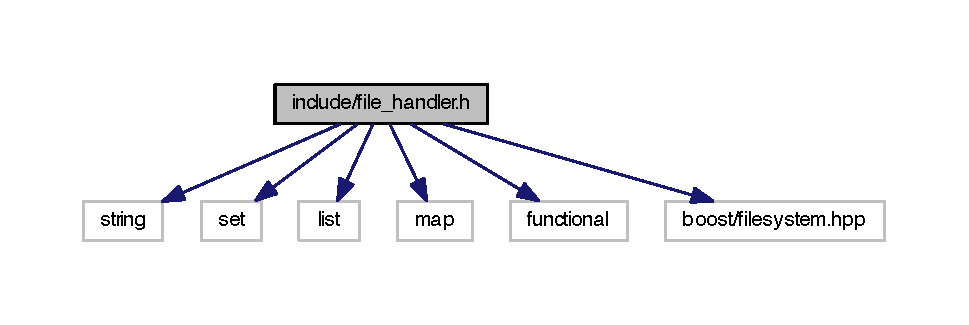
\includegraphics[width=350pt]{file__handler_8h__incl}
\end{center}
\end{figure}
\subsection*{Classes}
\begin{DoxyCompactItemize}
\item 
struct \hyperlink{structdfr_1_1file__data}{dfr\+::file\+\_\+data}
\item 
class \hyperlink{classdfr_1_1file__handler}{dfr\+::file\+\_\+handler}
\end{DoxyCompactItemize}


\subsection{Detailed Description}
This header manipulates file\textquotesingle{}s metadata and performs operations over it. 
\hypertarget{file__hash_8h}{}\section{include/file\+\_\+hash.h File Reference}
\label{file__hash_8h}\index{include/file\+\_\+hash.\+h@{include/file\+\_\+hash.\+h}}
{\ttfamily \#include $<$string$>$}\\*
Include dependency graph for file\+\_\+hash.\+h\+:\nopagebreak
\begin{figure}[H]
\begin{center}
\leavevmode
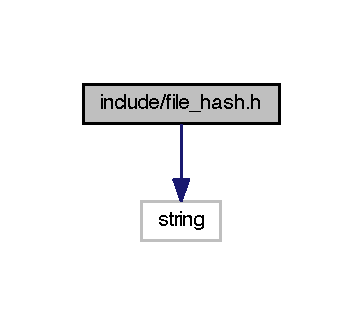
\includegraphics[width=174pt]{file__hash_8h__incl}
\end{center}
\end{figure}
\subsection*{Classes}
\begin{DoxyCompactItemize}
\item 
class \hyperlink{classdfr_1_1hash}{dfr\+::hash}
\end{DoxyCompactItemize}


\subsection{Detailed Description}
This file includes function to computes hash for the files at specified path. 
%--- End generated contents ---

% Index
\backmatter
\newpage
\phantomsection
\clearemptydoublepage
\addcontentsline{toc}{chapter}{Index}
\printindex

\end{document}
